\documentclass[handout]{beamer}
%\documentclass{beamer}
{
\usepackage{fullpage}
\usepackage{hyperref}
\usepackage{amssymb} 
}
\usepackage{pgf,pgfarrows,pgfnodes,pgfautomata,pgfheaps,pgfshade}
\usepackage{amsmath,amscd,amssymb}
\usepackage{colortbl}
\usepackage{tikz,pgf,pifont}
\usepackage{mathtools}
\usepackage{pbox}

\usepackage{lstlisting-llvm}
\usepackage[numbered]{mcode}
\usepackage{listings}
\lstloadlanguages{Matlab}
\lstdefinestyle{mcode}{language=MATLAB,escapechar=&}

\usepackage{xcolor}
\usepackage{textcomp}
\usepackage{pgfpages}
\usepackage{hologo}

%\pgfpagesuselayout{4 on 1}[a4paper, border shrink=5mm, landscape]



%\usepackage[latin1]{inputenc}
\usepackage[english]{babel}

  \usetheme{Boadilla}    % Very nice with fewer sections/sub and numbering
  % \usetheme{CambridgeUS}  % Sections and red white + numbers
  % \usetheme{Warsaw}      % Good one no numbers though
  % \usetheme{Darmstadt}   % no University and name
   \setbeamercovered{transparent}
  % \useoutertheme[subsection=true,footnote=false]{miniframes}
  \setbeamertemplate{navigation symbols}{}
  \usecolortheme{crane}

\usepackage{amsmath, amssymb, amsfonts, amsthm,
  verbatim, fancyhdr, graphicx, array, latexsym,
  color, listings, afterpage, epsfig, boxedminipage, 
  fancybox}
\usepackage{amsfonts,amsbsy}


%\usepackage[emtex]{changebar}
%\usepackage{mathptm}  % times+ math
%\usepackage{natbib}
%\usepackage{epsf}
%\usepackage{epsfig}
%\usepackage{rotate}
%\usepackage{amsmath}
%\usepackage{ifthen}
%\usepackage[english]{babel}
% or whatever
%\usepackage[latin1]{inputenc}

% or whatever 
\newcommand{\ud}{\mathrm{d}}
\newcommand{\commentout}[1]{}
\newcommand{\mybox}[1]{\hbox to 0.6\textwidth{#1\hss}}
\newcommand{\pmat}[1]{\begin{pmatrix}#1\end{pmatrix}} 
\newcommand{\red}[1]{\textcolor{red}{#1}}
\newcommand{\blue}[1]{\textcolor{blue}{#1}}
\newcommand{\brown}[1]{\textcolor{brown}{#1}}
\newcommand{\green}[1]{\textcolor{green}{#1}}
\newcommand{\purple}[1]{\textcolor{purple}{#1}}
\newcommand{\gray}[1]{\textcolor{gray}{#1}}


\newcommand{\pder}[2]{\frac{\partial #1}{\partial #2}}
 \newcommand{\norm}[2]{\ensuremath{\| #1 \|_{#2}}}
 \newcommand{\seq}[1]{\ensuremath{\left\{ #1 \right\}}}
 \newcommand{\ipt}[2]{\ensuremath{\left\langle#1,#2\right\rangle}}
 \newcommand{\vbblock}[3]{\ensuremath{\left(\begin{array}{c}\!\!\!#1\\\!\!\!#2\\\!\!\!#3\end{array}\!\!\!\right)}}

 \newcommand{\bblock}[9]{\ensuremath{\left(\begin{array}{ccc}#1&#2&#3\\#4&#5&#6\\#7&#8&#9\end{array}\right)}}
 \def \R{\bb{R}}\def \C{\bb{C}}\def \Z{\bb{Z}}\def \N{\bb{N}}
 \def \a{{\bf a}}
 \def \b{{\bf b}}
 \def \c{{\bf c}}
 \def \d{{\bf d}}
 \def \e{{\bf e}}
 \def \f{{\bf f}}
 \def \g{{\bf g}}
 \def \k{{\bf k}}
 \def \m{{\bf m}}
 \def \n{{\bf n}}
 \def \p{{\bf p}}
 \def \q{{\bf q}}
 \def \r{{\bf r}}
 \def \s{{\bf s}}
 \def \t{{\bf t}}
 \def \u{{\bf u}}
 \def \vv{{\bf v}}
 \def \w{{\bf w}}
 \def \x{{\bf x}}
 \def \y{{\bf y}}
 \def \z{{\bf z}}
 \def \rh{{\alert{h}}}
\def \M{{\cal M}}
\def \L{{\cal L}}
 \def \blambda{{\boldsymbol{\lambda}}}%works with package amsbsy
\newcommand{\hnorm}[2]{\ensuremath{| #1 |_{#2}}}
\newcommand{\ip}[2]{\ensuremath{\left(#1,#2\right)}}



\definecolor{Brown}{cmyk}{0,0.81,1,0.60}
\definecolor{Green}{rgb}{0.516, 0.5976, 0.480}
\definecolor{OliveGreen}{cmyk}{0.64,0,0.95,0.40}
\definecolor{CadetBlue}{rgb}{0.17,0.30,0.547}
\definecolor{Red}{rgb}{0.684,0.156,0.32}
\lstset{
  language=matlab,
  basicstyle=\ttfamily,
  frame=ltrb,
  framesep=5pt,
  basicstyle=\scriptsize,
  stringstyle=\ttfamily\color{Brown}\bfseries,
  commentstyle=\ttfamily\color{Green}\bfseries,
  keywordstyle=\ttfamily\color{CadetBlue}\bfseries,
  identifierstyle=\ttfamily, 
  tabsize=2,
  showstringspaces=true,
  numbers=none
}


%%%%%%%%%%%%%%%%%%%%%%%%%%%%%%%%%%%%%%%%%%%%%%%%%%%%%%%%%%%%%%%%%%%%%%
%%%%%%%%%%%%%%%%%%%%%%%%%%%%%%%%%%%%%%%%%%%%%%%%%%%%%%%%%%%%%%%%%%%%%%
%%%%%%%%%%%%%%%%%%%%%%%%%%%%%%%%%%%%%%%%%%%%%%%%%%%%%%%%%%%%%%%%%%%%%%

% slide 1:
% ========

% title and affiliation

\title[PDE LAB2, 2016]{Master of Science on Computational Science}



\author[Dr. Drosos Kourounis \& Hardik Kothari (TA)] % (optional, use only with lots of authors)
{\textbf{Institute of Computational Science}}
% - Give the names in the same order as the appear in the paper.
% - Use the \inst{?} command only if the authors have different
%   affiliation.

\institute[ICS] % (optional, but mostly needed)
{
Dr. Drosos Kourounis \& Hardik Kothari (TA)
}
% If you have a file called "university-logo-filename.xxx", where xxx
% is a graphic format that can be processed by latex or pdflatex,
% resp., then you can add a logo as follows:


%\pgfdeclareimage[height=1.0cm]{university-logo}{uoi}
%\logo{\pgfuseimage{university-logo}}

% - Use the \inst command only if there are several affiliations.
% - Keep it simple, no one is interested in your street address.

\date[3 Oct,  2016]{3 Oct, 2016, LAB2}

\usefonttheme{serif}


\AtBeginSubsection[]
{
  \begin{frame}<beamer>
    \frametitle{Outline}
    \tableofcontents[currentsection,currentsubsection]
  \end{frame}
}
\setbeamertemplate{footline}
{
  \begin{beamercolorbox}[colsep=1.5pt]{upper separation line foot}
  \end{beamercolorbox}
  \begin{beamercolorbox}[ht=2.5ex,dp=1.125ex,%
    leftskip=.3cm,rightskip=.3cm plus1fil]{title in head/foot}%
    \leavevmode{\usebeamerfont{title in head/foot}
      \insertsection \hfill \insertsubsection\ \hfill \insertshorttitle}%
  \end{beamercolorbox}%
  \begin{beamercolorbox}[colsep=1.5pt]{lower separation line foot}
  \end{beamercolorbox}
}



\begin{document}


\begin{frame}
  \titlepage
\end{frame}

\section{Finite Elements in 2D and 3D}


\begin{frame}
\frametitle{Interpolation in one dimension (1D)}
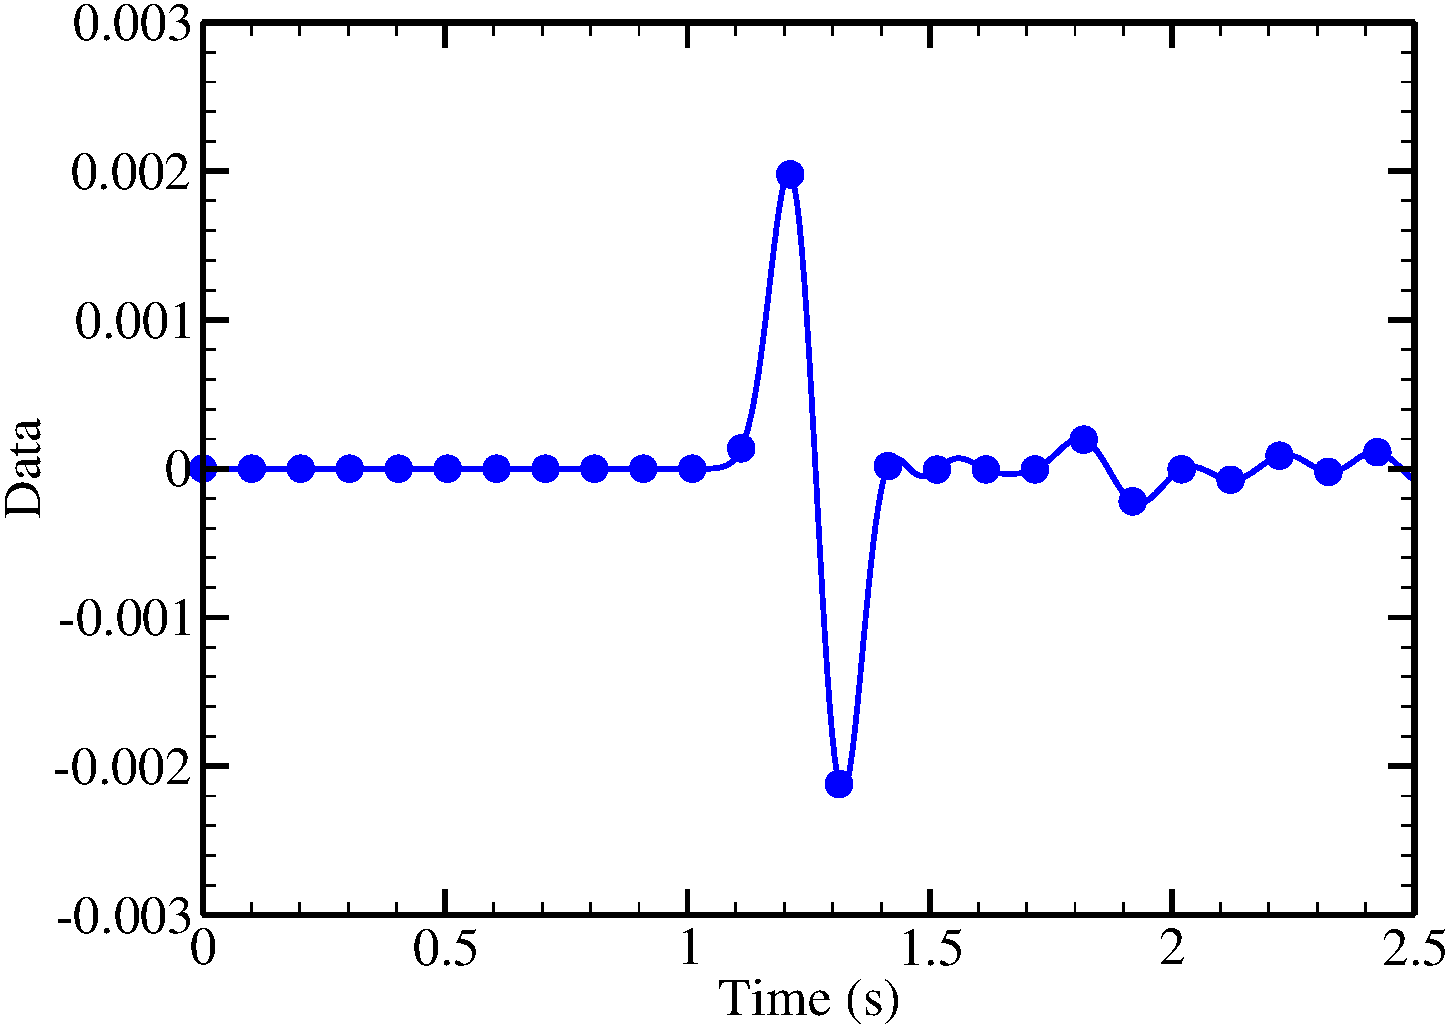
\includegraphics[width=0.8\textwidth]{FEM1D.pdf}
\end{frame}

\begin{frame}
\frametitle{Finite Elements in one dimension (1D)}
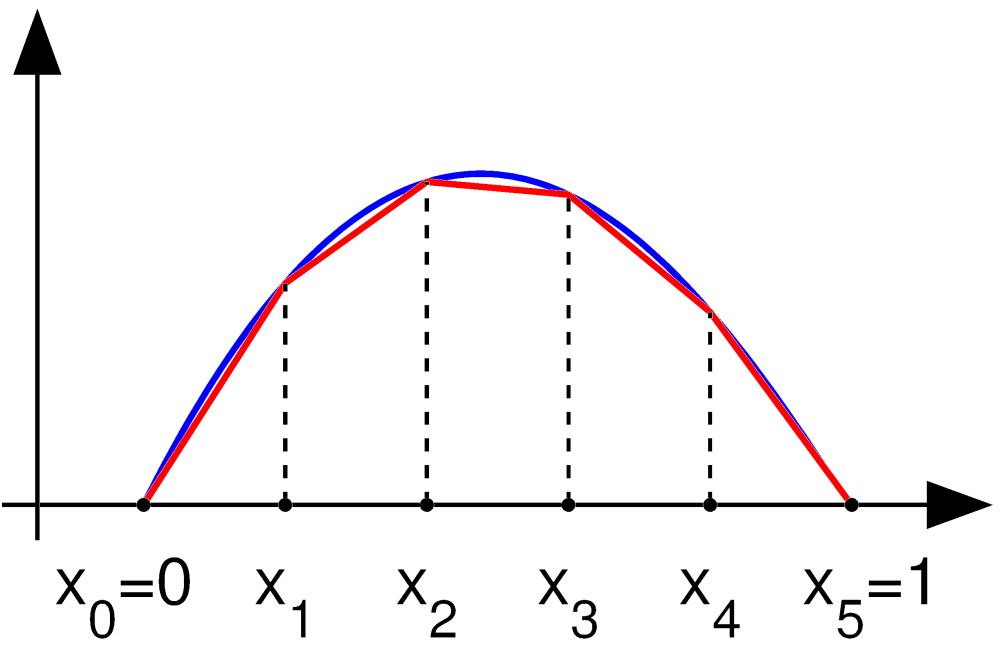
\includegraphics[width=0.8\textwidth]{FiniteElements1D.png}
\end{frame}


\begin{frame}
\frametitle{2D and 3D Finite Elements}
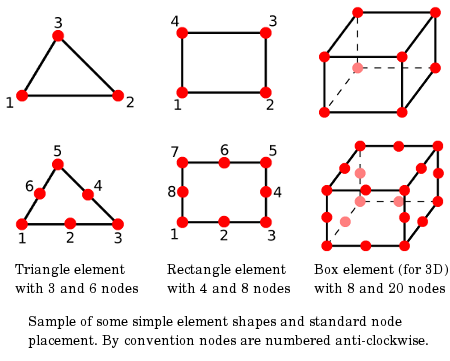
\includegraphics[width=0.8\textwidth]{FiniteElements.png}
\end{frame}


\begin{frame}
\frametitle{The 3D case can be very challenging}
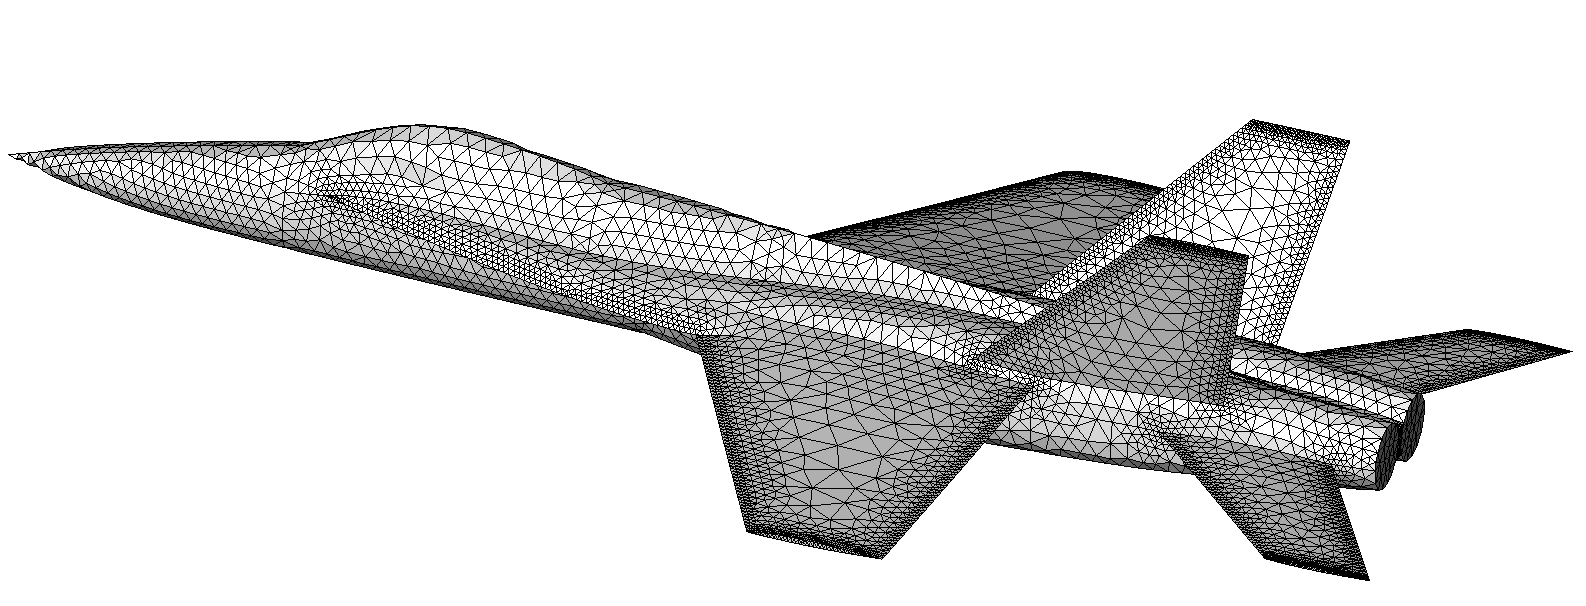
\includegraphics[width=\textwidth]{F17.png}
\end{frame}

\begin{frame}
\frametitle{Mapping to the reference element 3D}
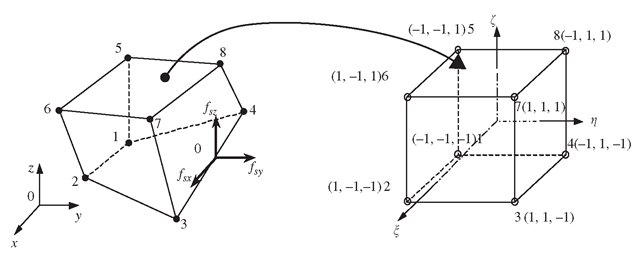
\includegraphics[width=0.8\textwidth]{FEmappingHex.png}
\end{frame}



\begin{frame}
\frametitle{Mapping to the reference in 2D}
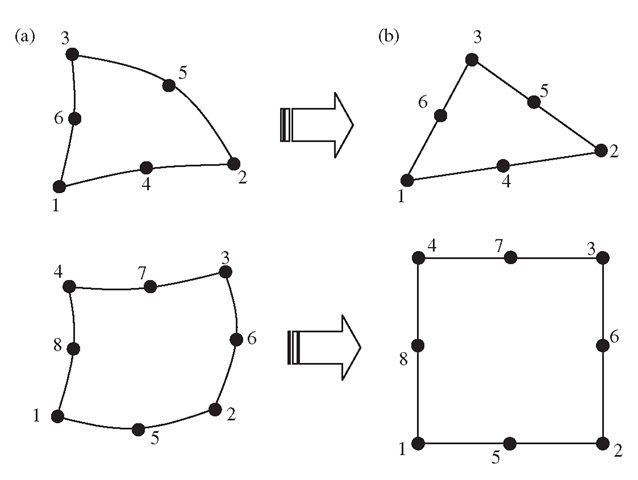
\includegraphics[width=0.8\textwidth]{FEmapping2D.png}
\end{frame}



\begin{frame}
\frametitle{Mapping to the reference in 3D}
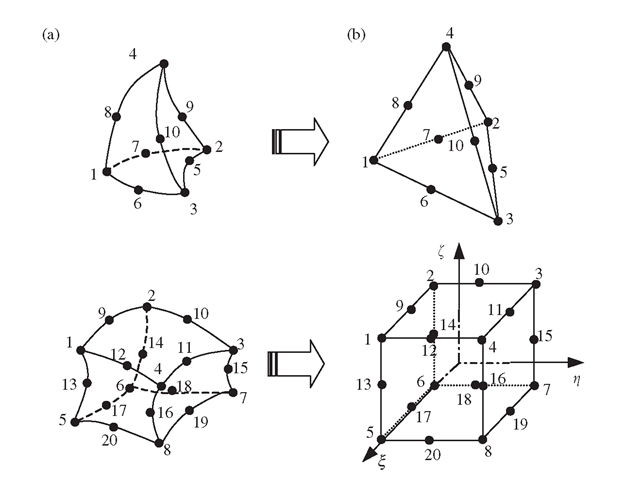
\includegraphics[width=0.8\textwidth]{FEmapping3D.png}
\end{frame}



\begin{frame}{The 2D quadrilateral element}
\begin{minipage}{0.45\textwidth}
\begin{figure}
     \begin{picture}(180,95)(-30,0)
     \thicklines
     \put(0,0){\line(1, 0){80}}
     \put(80,0){\line(0, 1){80}}
     \put(80,80){\line(-1, 0){80}}
     \put(0,0){\line(0, 1){80}}

     \put(5,5){1}
     \put(70,5){2}
     \put(70,70){3}
     \put(5,70){4}


     \put(40,40){\vector(1, 0){50}}
     \put(40,40){\vector(0, 1){50}}
     \put(100,40){$\xi$}
     \put(40,100){$\eta$}
     \put(28,30){(0,0)}

     \put(-15,-15){(-1,-1)}
     \put(70,-15){(1,-1)}
     \put(-15,90){(-1,1)}
     \put(70,90){(1,1)}
     \end{picture}
\end{figure}
\end{minipage}
\begin{minipage}{0.45\textwidth}
\begin{align*}
N_1 &= \frac{1}{4}(1 - \xi)(1 - \eta) \\
N_2 &= \frac{1}{4}(1 + \xi)(1 - \eta) \\ 
N_3 &= \frac{1}{4}(1 + \xi)(1 + \eta) \\
N_4 &= \frac{1}{4}(1 - \xi)(1 + \eta) \\
N_i &= \frac{1}{4}(1 + \xi_i\xi)(1 + \eta_i\eta)
\end{align*}
\end{minipage}
\end{frame}


\begin{frame}{The 2D quadrilateral element $\ldots$}
Any unknown field $u$ as well as the coordinates $(x, y)$
may be expressed as functions of $(\xi, \eta)$ as
\begin{align*}
u   &= N_1 u_1 + N_2 u_2 + N_3 u_3 + N_4 u_4 \\
x   &= N_1 x_1 + N_2 x_2 + N_3 x_3 + N_4 x_4 \\
y   &= N_1 y_1 + N_2 y_2 + N_3 y_3 + N_4 y_4.
\end{align*}
Now suppose $f = f(x,y)=f(x(\xi, \eta),y(\xi, \eta))$. Using the 
chain rule of differentiation, we have
\begin{align*}
\pder{f}{\xi}   &= \pder{f}{x}\pder{x}{\xi} + \pder{f}{y}\pder{y}{\xi} \\
\pder{f}{\eta}  &= \pder{f}{x}\pder{x}{\eta} + \pder{f}{y}\pder{y}{\eta} \\
\end{align*}

\end{frame}

\begin{frame}{The 2D quadrilateral element $\ldots$}
\begin{align*}
\pmat{ \pder{f}{\xi} \\ \\
   \pder{f}{\eta}  
}
=
J
\pmat{ \pder{f}{x} \\ \\
   \pder{f}{y}  
}&, \quad
J=
\pmat{ \pder{x}{\xi}  & \pder{y}{\xi} \\ \\
       \pder{x}{\eta} & \pder{y}{\eta}
}
\\ \\
\pmat{ \pder{f}{x} \\ \\
   \pder{f}{y}  
}
=
J^{-1}
\pmat{ \pder{f}{\xi} \\ \\
   \pder{f}{\eta}  
}&, \quad
dx  dy = |J|\; d\xi  d\eta
\end{align*}

\end{frame}

\begin{frame}{The 2D quadrilateral element $\ldots$}
\begin{align*}
J = \pmat{ J_{11} & J_{12} \\ J_{21} & J_{22} }
\end{align*}
\begin{align*}
J_{11}&=\frac{1}{4} 
\left ( 
  -(1-\eta) x_1 + (1-\eta) x_2 + (1+\eta) x_3 - (1 + \eta) x_4
\right ) \\
J_{12}&=\frac{1}{4} 
\left ( 
  -(1-\eta) y_1 + (1-\eta) y_2 + (1+\eta) y_3 - (1 + \eta) y_4
\right ) \\
J_{21}&=\frac{1}{4} 
\left ( 
  -(1-\xi) x_1 - (1+\xi) x_2 + (1+\xi) x_3 + (1 - \xi) x_4
\right ) \\
J_{22}&=\frac{1}{4} 
\left ( 
  -(1-\xi) y_1 - (1+\xi) y_2 + (1+\xi) y_3 + (1 - \xi) y_4
\right )
\end{align*}

\end{frame}

\begin{frame}{2D integrals}
Gaussian quadrature in 1D: $n$ points can integrate exactly a polynomial
of degree equal to $2 n - 1$
\begin{align*}
I &= \int_{-1}^1 f(\xi) d \xi  \\
I &\approx \sum_{k=1}^n w_k f(\xi_k) \\
\end{align*}


Gaussian quadrature in 2D
\begin{align*}
I &= \int_{-1}^1 \int_{-1}^1 f(\xi, \eta) d \xi \; d \eta \\
I &\approx \sum_{k_1=1}^n \sum_{k_2=1}^n w_{k_1} w_{k_2} f(\xi_{k_1}, \eta_{k_2}) \\
\end{align*}

\end{frame}

\begin{frame}{2D integrals $\ldots$}
Integrating the Laplacian on the reference element
\begin{align*}
I &= \int_{\Omega} \nabla N_i(x,y) \cdot \nabla N_j(x,y) d \Omega \\ \\
I &= \int_{\Omega_0} J^{-1} \nabla N_i (\xi, \eta) \cdot J^{-1}\nabla N_j (\xi, \eta) |J| d \Omega_0 \\ \\
I &= \int_{-1}^1 \int_{-1}^1 J^{-1} \nabla N_i(\xi, \eta) \cdot J^{-1}\nabla N_j(\xi, \eta) |J| d \xi \; d \eta \\ \\
I &\approx \sum_{k_1=1}^n \sum_{k_2=1}^n w_{k_1} w_{k_2} J^{-1}_{k_1,k_2} \nabla N_i(\xi_{k_1}, \eta_{k_2}) \cdot J^{-1}_{k_1,k_2} \nabla N_j(\xi_{k_1}, \eta_{k_2}) |J_{k_1,k_2}|\\
\end{align*}

\end{frame}

\begin{frame}{}
\begin{center}
$\displaystyle M = \int_V N_i N_j d V$
\lstinputlisting[language=matlab,firstnumber=1,basicstyle=\ttfamily\scriptsize]{Msymbolic.m}
\end{center}
\end{frame}


\begin{frame}{}
\begin{center}
$\displaystyle K = \int_V \nabla N_i \cdot \nabla N_j d V$
\lstinputlisting[language=matlab,firstnumber=1,basicstyle=\ttfamily\scriptsize]{Ksymbolic.m}
\end{center}
\end{frame}

%\begin{frame}{}
%\begin{center}
%$\displaystyle I = \int_V \nabla N_i \cdot \nabla N_j d V$
%\lstinputlisting[language=matlab,firstnumber=1,basicstyle=\ttfamily\scriptsize]{Msymbolic.m}
%\end{center}
%\end{frame}



\end{document}
